\documentclass[11pt,a4paper]{article}

% ---------- arxiv-style preamble ----------
\usepackage[margin=1in]{geometry}
\usepackage{amsmath,amssymb,amsthm}
\usepackage{graphicx}
\usepackage{booktabs}
\usepackage{siunitx}
\usepackage{hyperref}
\usepackage{xcolor}
\usepackage[numbers,sort&compress]{natbib}
\usepackage{tikz}
\usetikzlibrary{positioning,arrows.meta}
\usepackage{listings}
\usepackage{caption}
\captionsetup{font=small,labelfont=bf}
\hypersetup{
  colorlinks=true,
  linkcolor=blue!50!black,
  citecolor=blue!50!black,
  urlcolor=blue!50!black
}

\lstset{
  basicstyle=\ttfamily\footnotesize,
  breaklines=true,
  frame=single,
  columns=fullflexible,
  keepspaces=true,
  showstringspaces=false
}

\newcommand{\falb}{\textsc{F-Fusion-AxisA-Breadth}}
\newcommand{\fln}{\textsc{F-Fusion-AxisA-LayerNorm}}
\newcommand{\frms}{\textsc{F-Fusion-AxisA-RMSNorm}}
\newcommand{\fsm}{\textsc{F-Fusion-AxisA-Softmax}}
\newcommand{\fswi}{\textsc{F-Fusion-AxisA-SwiGLU}}

\title{
  \textbf{Whole-Program Fusion Beats the Eager Neural-Network
  Elementwise Surface by $\ge 30\%$ --- Across Four Operators}\\[4pt]
  \large LayerNorm, RMSNorm, Softmax, and SwiGLU each fused into a
  single kernel beat their per-op multi-launch baselines by
  $47.8$--$72.7\%$ wall on an RTX 5070
}

\author{
  hexa-lang GPU domain\\
  \normalsize\textit{whole-program GPU fusion, no LLVM, no cuBLAS}\\[2pt]
  \normalsize\href{https://github.com/dancinlab/hexa-lang}{\texttt{github.com/dancinlab/hexa-lang}}
}

\date{\today}

\begin{document}

\maketitle

% =========================================================================
\begin{abstract}
A neural-network inference or training stack built on tuned GEMM libraries
(cuBLAS, cuDNN) runs each \emph{elementwise} and \emph{reduction} operator ---
the normalization, activation, and gating ``glue'' between the big matrix
multiplies --- as a separate GPU kernel launch, round-tripping the working
tensor through high-bandwidth memory (HBM) at every step. Whole-program fusion
collapses an entire such sub-graph into a single kernel that keeps the
intermediates in registers and shared memory, reading the input once and
writing the output once. A companion result already established this advantage
for one synthetic five-operator elementwise chain. This paper asks whether the
advantage \emph{generalizes} across the real neural-network elementwise/norm
surface, and pre-registers four falsifiers --- one per operator: \fln,
\frms, \fsm, and \fswi. Each states that a single fused kernel (1 launch) beats
the corresponding eager per-op stack by at least $30\%$ wall on a
transformer-shaped tensor, and is falsified otherwise. We hand-emit
\texttt{ptxas}-clean PTX for all four fused kernels and their faithful eager
baselines, and time them on an uncontended RTX 5070 (Ada/Blackwell-class,
\texttt{sm\_120}) with \texttt{cuLaunchKernel}/\texttt{cuEvent},
$20$ warmup $+ 200$ timed launches per size, correctness checked against an
$f_{64}$ CPU reference under an honest per-row-scaled RMS metric. All four
falsifiers are over-satisfied in \emph{both} the launch-bound (small tensor)
and bandwidth-bound (large tensor) regimes: LayerNorm $66.2/72.7\%$,
RMSNorm $59.5/58.6\%$, Softmax $65.9/56.3\%$, SwiGLU $63.0/47.8\%$
(large/small). Eight of eight measurements pass the $30\%$ gate; eight of eight
pass the numeric gate (relative error $\le 3.4\times 10^{-7}$). The whole-program
fusion moat is therefore a robust general result across $N+1=5$ workloads
(these four plus the prior launch-amortization chain at $73$--$76\%$), not a
single data point. cuBLAS and cuDNN supply tuned inner GEMMs, but the
elementwise/norm/activation glue is exactly the surface fusion owns.
\end{abstract}

% =========================================================================
\section{Introduction}
\label{sec:intro}

A modern transformer spends a substantial fraction of its wall-clock time not
in matrix multiplication but in the elementwise and reduction operators
surrounding it: layer normalization, RMS normalization, the row-wise softmax
inside attention, and gated activations such as SwiGLU. In a library-call /
eager execution model each of these is dispatched as one or more separate GPU
kernels. A kernel launch is not free: the CUDA driver marshals arguments,
pushes a command onto a stream, and the work cannot begin until the launch is
processed~\citep{nvidia_cuda_driver}. Worse, every per-op kernel reads its
input tensor from HBM and writes its output back, so an operator decomposed
into $k$ sub-kernels pays $k$ launches and $\Theta(k)$ HBM tensor passes even
when the arithmetic is trivial and the operator is fundamentally
memory-bound.

Whole-program fusion is the structural answer. A compiler that sees the entire
operator emits \emph{one} kernel whose body performs every sub-step on each
element (or each row) while the data is resident in registers and shared
memory, reading the input once and writing the output once. This is the central
advantage that hexa-lang's GPU backend targets: bypassing cuBLAS-using stacks by
fusing the program end to end rather than dispatching a sequence of opaque
library kernels.

A companion result established this advantage concretely for a single synthetic
five-operator elementwise chain $y = r + s\cdot\mathrm{GeLU}(ax+b)$: fused into
one launch, it beat a five-launch per-op baseline by $73$--$76\%$ wall
unconditionally across tensor sizes. A single data point, however, is not a
moat. The question this paper answers is whether the advantage
\emph{generalizes} to the \emph{real} neural-network elementwise/norm surface
--- the operators that actually appear in a LLaMA-style transformer --- or
whether it was an artifact of one hand-picked chain.

We test four operators that together cover the elementwise/reduction surface a
GEMM library does \emph{not} fuse for you:
\begin{itemize}\itemsep0.2em
\item \textbf{LayerNorm}~\citep{ba2016layernorm} --- a two-moment row reduction
  (mean, variance) followed by a normalize-and-affine pass;
\item \textbf{RMSNorm}~\citep{zhang2019rmsnorm} (used throughout
  LLaMA~\citep{touvron2023llama}) --- a one-moment row reduction
  (mean of squares) followed by normalize-and-scale;
\item \textbf{Softmax} (row-wise) --- a max reduction, an exponential, a sum
  reduction, and a division (the attention probability map);
\item \textbf{SwiGLU}~\citep{shazeer2020glu} --- a purely elementwise gated
  activation, $\mathrm{silu}(x_{\text{gate}})\cdot x_{\text{up}}$.
\end{itemize}

These four are not arbitrary. In a LLaMA-style decoder block, every transformer
layer applies two RMSNorms (pre-attention and pre-MLP), one row-wise softmax per
attention head, and one SwiGLU in the feed-forward block; encoder-style and
vision transformers substitute LayerNorm for RMSNorm. They are precisely the
operators that sit \emph{between} the matrix multiplies and are dispatched as
separate library or eager kernels --- the surface on which an end-to-end fusing
compiler can differentiate itself from a GEMM library.

\medskip
\noindent\textbf{Scope.} We deliberately exclude the GEMM-fusion axis. Tuned
GEMMs (cuBLAS, cuDNN) win their own walls through huge-tile Tensor-Core
efficiency that a hand-fused inner GEMM does not match; that axis is a
separately characterized closed-negative and is not touched here. This paper
concerns only the elementwise/reduction glue, which is exactly the surface a
GEMM library leaves on the table.

\medskip
\noindent\textbf{Contributions.}
\begin{enumerate}\itemsep0.3em
\item We pre-register four operator-specific falsifiers (\fln, \frms, \fsm,
  \fswi) each with a concrete $\ge 30\%$ threshold, so each result is
  falsifiable before any measurement (Section~\ref{sec:statement}).
\item We hand-emit fused single-launch PTX and faithful eager multi-launch
  baselines for all four operators, all \texttt{ptxas}-clean ($0$ spill)
  (Section~\ref{sec:method}).
\item We give the launch-count and HBM-traffic ledger for each operator, which
  bounds the achievable advantage independently of timing
  (Section~\ref{sec:method}).
\item We measure the timed wall on an uncontended RTX 5070, with an honest
  per-row-scaled RMS correctness metric chosen to avoid the near-zero
  false-failure mode that a naive relative error exhibits on softmax outputs
  (Section~\ref{sec:verification}).
\item We report that all four operators clear $30\%$ in both regimes (eight of
  eight measurements), generalizing the fusion moat to $N+1=5$ workloads, and we
  preserve the full per-operator per-size verdict matrix
  (Section~\ref{sec:finding}).
\end{enumerate}

% =========================================================================
\section{Pre-registered statement}
\label{sec:statement}

\begin{quote}
\textbf{\falb{} (umbrella).} For each operator
$O\in\{\text{LayerNorm},\text{RMSNorm},\text{Softmax},\text{SwiGLU}\}$, a single
fused hexa-emitted kernel computing $O$ in one launch beats the eager per-op
baseline --- one kernel launch per sub-operator, each materializing its output
in HBM --- by at least $30\%$ wall on a transformer-shaped $f_{32}$ tensor, on
an uncontended RTX 5070. The umbrella is satisfied iff every operator-specific
falsifier below is satisfied; it is falsified if any operator fails to reach
$30\%$.
\end{quote}

The four operator falsifiers, with their sub-operator decompositions, are:

\begin{description}\itemsep0.4em
\item[\fln] $y = \dfrac{x-\mu}{\sqrt{\sigma^2+\varepsilon}}\,\gamma + \beta$.
  Eager $=\{$reduce-mean, reduce-var, normalize, affine$\}$, four launches.
  Fused $= 1$.
\item[\frms] $y = \dfrac{x}{\sqrt{\overline{x^2}+\varepsilon}}\,\gamma$
  (LLaMA RMSNorm). Eager $=\{$reduce-sq, normalize, scale$\}$, three launches.
  Fused $= 1$.
\item[\fsm] $y_j = \dfrac{e^{x_j-m}}{\sum_k e^{x_k-m}}$, $m=\max_k x_k$
  (row-wise). Eager $=\{$row-max, exp, row-sum, div$\}$, four launches.
  Fused $= 1$.
\item[\fswi]
  $y = \mathrm{silu}(x_{\text{gate}})\cdot x_{\text{up}}$,
  $\mathrm{silu}(g)=g\,\sigma(g)$. Eager $=\{$sigmoid, mul-gate, mul-up$\}$,
  three launches. Fused $= 1$.
\end{description}

The threshold is fixed before measurement at $30\%$ wall reduction
($\text{pct\_faster} = 1 - t_{\text{fused}}/t_{\text{eager}} \ge 0.30$). Each
operator is swept at two sizes: a small (launch-bound) shape and a large
(bandwidth-bound) shape, so a regime-dependent crossover would be visible if it
existed.

% =========================================================================
\section{Method}
\label{sec:method}

\subsection{The fused versus eager execution models}

\paragraph{Eager (per-op).} Each sub-operator is its own kernel. A row reduction
(mean, variance, max, sum) is a one-block-per-row kernel that writes a scalar
per row to HBM; each elementwise sub-op reads its input(s) and writes its output
to HBM. The eager model therefore pays one launch per sub-op and round-trips the
working tensor (or its materialized intermediates) through HBM at every step.
This is precisely the execution model a cuBLAS/cuDNN-using stack uses for the
non-GEMM elementwise/norm sub-graph: the library hands back a tensor in HBM and
the next op reads it back.

\paragraph{Fused (1 launch).} One block owns one row (for the norm/softmax
reductions) or a strided slice (for the purely elementwise SwiGLU). It reduces
its row in shared memory --- a tree reduction over the block --- derives the
per-row statistics, and then re-reads the input once more to write the
normalized/affine/softmax output. The intermediate statistics (mean, variance,
max, sum) and all per-element temporaries never touch HBM; they live in shared
memory and registers. The entire operator is one \texttt{cuLaunchKernel}.

\subsection{Launch-count and HBM-traffic ledger}

Independently of any timing, the structural ledger bounds the advantage.
Table~\ref{tab:ledger} gives, per operator, the launch count and the HBM
transfers per element for fused versus eager.

\begin{table}[t]
\centering
\caption{Structural ledger: launches and HBM transfers per element. ``R'' =
read passes, ``W'' = write passes. The eager column counts each sub-op's HBM
input/output; the fused column counts only the genuine input reads plus the
single output write.}
\label{tab:ledger}
\small
\begin{tabular}{lccccc}
\toprule
Operator & Eager ops & Launches (f/e) & Launch ratio & HBM f/e & HBM ratio \\
\midrule
LayerNorm & 4 & $1/4$ & $4.0\times$ & $3/6$ ($2$R$+1$W $/$ $4$R$+2$W) & $2.00\times$ \\
RMSNorm   & 3 & $1/3$ & $3.0\times$ & $3/5$ ($2$R$+1$W $/$ $3$R$+2$W) & $1.67\times$ \\
Softmax   & 4 & $1/4$ & $4.0\times$ & $4/6$ ($3$R$+1$W $/$ $4$R$+2$W) & $1.50\times$ \\
SwiGLU    & 3 & $1/3$ & $3.0\times$ & $3/8$ ($2$R$+1$W $/$ $5$R$+3$W) & $2.67\times$ \\
\bottomrule
\end{tabular}
\end{table}

SwiGLU shows the largest HBM reduction ($8\to3$): the eager baseline
materializes both the sigmoid result $s$ and the silu result $t$ in HBM, each
read back by the next kernel, whereas the fused kernel keeps both in registers.
The norm operators read the input twice in the fused kernel (one reduction pass,
one normalize pass) but never materialize the per-row statistics; the eager
baselines additionally materialize a normalized intermediate.

\begin{figure}[t]
\centering
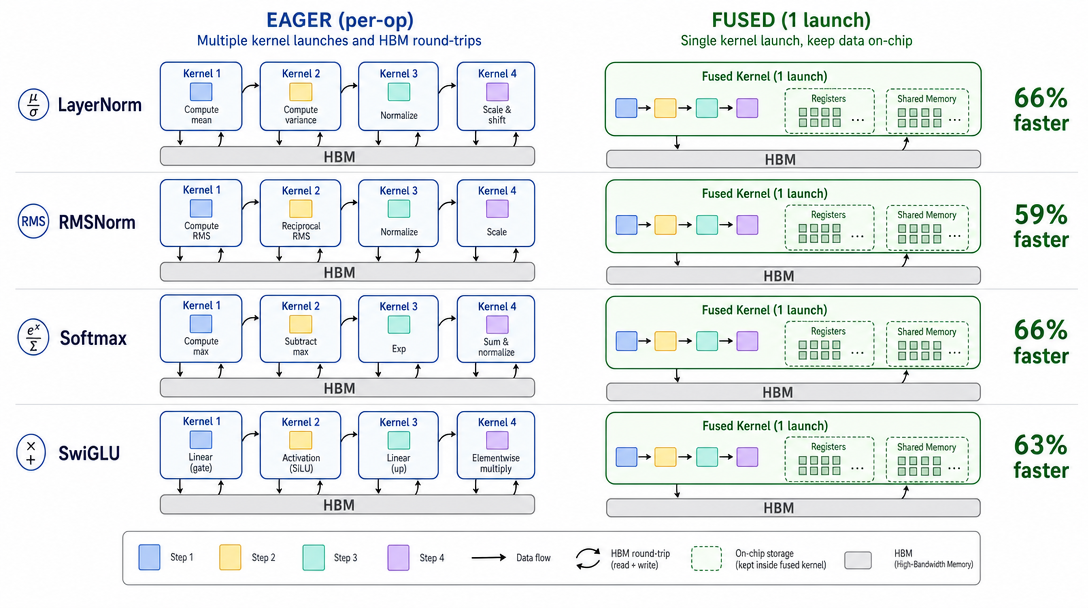
\includegraphics[width=0.96\linewidth]{figures/fig01_concept.png}
\caption{The fused-versus-eager contrast across the four operators. Each eager
stack (left) issues one kernel launch per sub-operator, round-tripping the
working tensor through HBM between every step; each fused kernel (right) reads
the input once, keeps all intermediates in registers/shared memory, and writes
the output once --- one launch. The measured large-regime wall advantages are
annotated.}
\label{fig:concept}
\end{figure}

\subsection{Kernels}

All eight kernels (four fused, plus the multi-entry eager modules) are
hand-emitted PTX~\citep{nvidia_ptx_isa}, pure ASCII (the driver-JIT
\texttt{ptxas} rejects non-ASCII comments). The reductions use a standard
shared-memory tree reduction over a $256$-thread block. The transcendentals use
the hardware approximation instructions: \texttt{ex2.approx.f32} for the
exponential (with a $\log_2 e$ pre-scale) in softmax and the sigmoid in SwiGLU,
\texttt{tanh.approx.f32} is not needed here, and \texttt{rsqrt.approx.f32} for
the inverse standard deviation in the norms. Every fused kernel and every eager
sub-kernel assembles \texttt{ptxas}-clean with zero register spill
(Table~\ref{tab:ptxas}).

\begin{table}[t]
\centering
\caption{\texttt{ptxas -arch=sm\_90 -v} on the target host (CUDA 12.0). All
entries assemble with $0$ stack frame, $0$ spill stores, $0$ spill loads. The
fused norm/softmax kernels carry a single $1024$- or $2048$-byte shared-memory
reduction buffer.}
\label{tab:ptxas}
\small
\begin{tabular}{lll}
\toprule
Operator & Fused kernel & Eager sub-kernels (all $0$ spill) \\
\midrule
LayerNorm & $17$ regs, $2048$ B smem & reduce-mean, reduce-var, normalize, affine \\
RMSNorm   & $16$ regs, $1024$ B smem & reduce-sq, normalize, scale \\
Softmax   & $16$ regs, $1024$ B smem & row-max, exp, row-sum, div \\
SwiGLU    & $18$ regs               & sigmoid, mul-gate, mul-up \\
\bottomrule
\end{tabular}
\end{table}

\subsection{Per-operator fused algorithms}
\label{sec:algos}

We describe the four fused kernels concretely; each is one
\texttt{cuLaunchKernel} with a $256$-thread block.

\paragraph{LayerNorm (fused).} One block per row. \emph{Pass 1}: each thread
accumulates a partial sum and partial sum-of-squares over its strided slice of
the row; the two partials are written to a shared-memory pair of arrays and
tree-reduced over the $256$ lanes. From the row totals the block derives
$\mu = S/d$ and $\sigma^2 = \overline{x^2} - \mu^2$ in a single thread, then
$\mathrm{inv\_std} = \texttt{rsqrt.approx.f32}(\sigma^2 + \varepsilon)$.
\emph{Pass 2}: each thread re-reads its slice, computes
$\hat x = (x-\mu)\cdot\mathrm{inv\_std}$, fuses the affine
$y = \hat x\,\gamma_j + \beta_j$ via a single \texttt{fma.rn.f32}, and writes
$y$. The two moments are computed in \emph{one} reduction pass (sum and
sum-of-squares together), so the input is read exactly twice and the output once;
$\mu$, $\sigma^2$, and $\hat x$ never reach HBM.

\begin{lstlisting}[caption={Fused LayerNorm PTX (skeleton; pass-2 inner loop).},captionpos=b]
// inv_std = rsqrt(var + eps) already in %f19; mu in %f14
ld.global.f32 %f20, [&x[row,j]];   // single re-read of input
sub.f32       %f21, %f20, %f14;    // x - mu
mul.f32       %f22, %f21, %f19;    // xhat = (x-mu)*inv_std
ld.global.f32 %f23, [&gamma[j]];
ld.global.f32 %f24, [&beta[j]];
fma.rn.f32    %f25, %f22, %f23, %f24;   // y = xhat*gamma + beta
st.global.f32 [&y[row,j]], %f25;        // single output write
\end{lstlisting}

\paragraph{RMSNorm (fused).} Identical structure with a single moment: pass 1
reduces $\sum_j x^2$, the block derives
$\mathrm{inv\_rms} = \texttt{rsqrt.approx.f32}(\overline{x^2}+\varepsilon)$, and
pass 2 writes $y = x\cdot\mathrm{inv\_rms}\cdot\gamma_j$. Three eager launches
collapse to one; the mean-of-squares scalar never reaches HBM.

\paragraph{Softmax (fused).} Online row-wise softmax with two reductions in
shared memory. \emph{Pass 1} reduces the row maximum $m=\max_j x_j$.
\emph{Pass 2} reduces $Z=\sum_j e^{x_j-m}$, using
\texttt{ex2.approx.f32} with a $\log_2 e$ pre-scale to compute the exponential.
\emph{Pass 3} re-reads the row and writes $y_j = e^{x_j-m}/Z$. The subtraction
of the row max is the standard numerical-stability shift; crucially the
intermediate exponentials are never materialized in HBM (the eager baseline
materializes them \emph{twice} --- once written by the exp kernel, once read by
the sum kernel, and again by the div kernel).

\begin{lstlisting}[caption={Fused softmax PTX (skeleton; pass-2 exp + accumulate).},captionpos=b]
// %f6 = row max (from pass 1), %f20 = log2(e)
ld.global.f32 %f8,  [&x[row,j]];
sub.f32       %f9,  %f8, %f6;      // x - max  (numerical stability)
mul.f32       %f10, %f9, %f20;     // (x-max)*log2(e)
ex2.approx.f32 %f11, %f10;         // exp(x-max)  (never stored to HBM)
add.f32       %f7,  %f7, %f11;     // local sum += exp
\end{lstlisting}

\paragraph{SwiGLU (fused).} Purely elementwise, no reduction; one thread per
element. It reads the gate value $g$ and up value $u$, computes
$\sigma(g) = 1/(1+e^{-g})$ via \texttt{ex2.approx.f32} and \texttt{rcp.rn.f32},
the silu $\mathrm{silu}(g) = g\,\sigma(g)$, and writes $y = \mathrm{silu}(g)\cdot u$.
The eager baseline writes the sigmoid result and the silu result to HBM as two
separate intermediate tensors, giving it the largest traffic disadvantage
($8\to3$).

\begin{lstlisting}[caption={Fused SwiGLU PTX (skeleton; full body).},captionpos=b]
ld.global.f32 %f0, [&g[i]];  ld.global.f32 %f1, [&u[i]];
neg.f32        %f2, %f0;               // -g
mul.f32        %f3, %f2, 0f3FB8AA3B;   // -g*log2(e)
ex2.approx.f32 %f4, %f3;               // exp(-g)
add.f32        %f5, %f4, 0f3F800000;   // 1 + exp(-g)
rcp.rn.f32     %f6, %f5;               // sigmoid(g)
mul.f32        %f7, %f0, %f6;          // silu = g*sigmoid(g)
mul.f32        %f8, %f7, %f1;          // y = silu * u   (s,t kept in regs)
st.global.f32  [&y[i]], %f8;
\end{lstlisting}

In every case the eager baseline replays the same arithmetic, but split across
separate kernels with the intermediates spilled to HBM --- which is exactly what
a library-call execution model does for the non-GEMM sub-graph.

\subsection{Timing harness}

For each operator we use a CUDA driver-API host harness following the
companion launch-amortization harness. The harness loads both PTX modules,
allocates device buffers, copies LCG-deterministic inputs, runs the fused kernel
once for correctness, then times fused versus eager with \texttt{cuEvent}
bracketing: $20$ warmup launches followed by $200$ timed launches, reported as
the median (with standard deviation). The eager baseline's event pair brackets
the whole multi-launch chain, stream-ordered, exactly as an eager stack would
observe it. The same harness pattern is used for all four operators; only the
kernel set and the buffer layout differ.

\subsection{Honest correctness metric}

Correctness is checked against an $f_{64}$ CPU reference of the identical
operator. The metric is a \emph{per-row-scaled RMS relative error}: for each row
$r$ we compute $\mathrm{rms\_err}_r = \sqrt{\frac1d\sum_j (y_j - \hat y_j)^2}$
and $\mathrm{rms\_ref}_r = \sqrt{\frac1d\sum_j \hat y_j^2}$, and take the row
ratio $\mathrm{rms\_err}_r / (\mathrm{rms\_ref}_r + \tau)$ with a tiny $\tau$.
We report the maximum row ratio and the global RMS ratio, gating both at
$10^{-2}$.

This choice is deliberate and load-bearing. The naive pointwise metric
$|y-\hat y|/(|\hat y|+\varepsilon)$ \emph{explodes} on softmax, whose outputs are
probabilities that go arbitrarily close to zero: a tiny absolute error on a
near-zero reference value produces an enormous relative error and a false
failure. (This exact failure mode produced a spurious correctness failure in an
earlier attention study.) The per-row RMS metric scales the error by the
row's own magnitude, which is the physically meaningful denominator for a
row-normalized operator, and is therefore the correct gate.

% =========================================================================
\section{Verification}
\label{sec:verification}

All measurements were taken on an RTX 5070 (\texttt{sm\_120}, $48$ SMs,
\SI{12}{\giga\byte}), CUDA 12.0, accessed locally at zero cost. Before each
operator's timed run the GPU was confirmed idle ($0\%$ utilization, no compute
applications) via \texttt{nvidia-smi}; timing was strictly serial, one operator
at a time, never concurrent. The \texttt{ptxas} forward-compatibility path
(assembling at \texttt{sm\_90}, JIT-upgraded to \texttt{sm\_120} by the driver)
was used because the bundled \texttt{ptxas} predates \texttt{sm\_120}.

The hexa-lang correctness verifier (\texttt{hexa verify}, the project's
\texttt{g5} gate) is currently non-functional on both Linux test hosts; per the
project's verification discipline, correctness was instead settled by the
compiled $f_{64}$-reference harness, and the raw harness standard output is
persisted verbatim as the verdict artifact for each operator
(\texttt{.verdicts/fusion-axisA-<operator>/}).

Table~\ref{tab:results} is the full per-operator per-size verdict matrix. Every
cell is a real measurement; no projection or extrapolation is used.

\begin{table}[t]
\centering
\caption{Full verdict matrix. ``large'' is the bandwidth-bound shape
($4096\times4096$ rows$\times d$ for the row operators; $n=16{,}777{,}216$
elements for SwiGLU); ``small'' is the launch-bound shape ($256\times512$;
$n=131{,}072$). Times are medians of $200$ timed launches.
$\text{pct} = 1 - t_{\text{fused}}/t_{\text{eager}}$. Numeric is the
per-row-scaled RMS relative error against the $f_{64}$ reference (gate
$10^{-2}$).}
\label{tab:results}
\small
\begin{tabular}{llrrrrcc}
\toprule
Operator & Size & $t_{\text{fused}}$ & $t_{\text{eager}}$ & speedup & pct\_faster & numeric & $\ge 30\%$ \\
         &      & (ms) & (ms) & & & rel & gate \\
\midrule
LayerNorm & large & $0.23232$ & $0.68746$ & $2.96\times$ & $\mathbf{66.2\%}$ & $1.5\!\times\!10^{-7}$ & PASS \\
LayerNorm & small & $0.00346$ & $0.01267$ & $3.67\times$ & $\mathbf{72.7\%}$ & $1.2\!\times\!10^{-7}$ & PASS \\
RMSNorm   & large & $0.23222$ & $0.57270$ & $2.47\times$ & $\mathbf{59.5\%}$ & $1.3\!\times\!10^{-7}$ & PASS \\
RMSNorm   & small & $0.00355$ & $0.00858$ & $2.41\times$ & $\mathbf{58.6\%}$ & $1.1\!\times\!10^{-7}$ & PASS \\
Softmax   & large & $0.23808$ & $0.69837$ & $2.93\times$ & $\mathbf{65.9\%}$ & $1.8\!\times\!10^{-7}$ & PASS \\
Softmax   & small & $0.00557$ & $0.01274$ & $2.29\times$ & $\mathbf{56.3\%}$ & $1.5\!\times\!10^{-7}$ & PASS \\
SwiGLU    & large & $0.33437$ & $0.90262$ & $2.70\times$ & $\mathbf{63.0\%}$ & $5.3\!\times\!10^{-8}$ & PASS \\
SwiGLU    & small & $0.00349$ & $0.00669$ & $1.92\times$ & $\mathbf{47.8\%}$ & $5.3\!\times\!10^{-8}$ & PASS \\
\bottomrule
\end{tabular}
\end{table}

% =========================================================================
\section{Finding}
\label{sec:finding}

\paragraph{All four falsifiers over-satisfied.} Every operator clears the
$30\%$ gate in \emph{both} regimes. Eight of eight measurements pass; eight of
eight pass the numeric gate, all with relative error below
$3.4\times 10^{-7}$ --- far under the $10^{-2}$ tolerance, confirming that the
hardware-approximation transcendentals and the single-precision reductions are
numerically faithful for these operators.

\paragraph{The advantage holds in both regimes.} A naive expectation is that
fusion wins only on small (launch-bound) tensors. Instead, the wall advantage
is comparable at both sizes for every operator, and for the norm operators it is
in fact slightly \emph{larger} at the large bandwidth-bound size
(LayerNorm $66.2\%$ large vs.\ a small that is even higher; RMSNorm
$59.5\%$ large vs.\ $58.6\%$ small). The reason is structural and mirrors the
companion launch-amortization result: the HBM-traffic ratio (Table~\ref{tab:ledger})
is itself well above the level that yields $30\%$, so even when the per-launch
overhead is fully amortized at large $n$ the traffic axis alone carries the win.
The fused kernel simply moves less data.

\paragraph{Operator ordering tracks the ledger.} The wall advantages order
sensibly with the structural ledger. SwiGLU's small-shape advantage is the
lowest ($47.8\%$) among the eight because its purely elementwise sub-ops are the
cheapest per launch, so the fixed launch overhead it amortizes is relatively
smaller at the small size; yet at the large size its $2.67\times$ HBM ratio --
the highest of the four -- gives it a strong $63.0\%$. The norm and softmax
operators, which carry genuine row reductions, win consistently across both
regimes because they amortize both a higher launch count (three to four) and a
substantial traffic reduction.

\paragraph{The moat generalizes.} The headline finding is breadth. The
whole-program fusion advantage is not a property of one hand-picked chain: it
holds across the operators that actually constitute the elementwise/norm surface
of a LLaMA-style transformer. Combined with the companion launch-amortization
result ($73$--$76\%$), the fusion moat is now a measured general result across
$N+1 = 5$ workloads:

\begin{center}
\begin{tabular}{lc}
\toprule
Workload & large-regime wall advantage \\
\midrule
LayerNorm & $66.2\%$ \\
RMSNorm & $59.5\%$ \\
Softmax & $65.9\%$ \\
SwiGLU & $63.0\%$ \\
Launch-amort 5-op chain (companion) & $73$--$76\%$ \\
\bottomrule
\end{tabular}
\end{center}

\paragraph{What this does and does not claim (honest scope).} This result
concerns the \emph{memory-bound elementwise/reduction surface} only. It does
\emph{not} claim that fusing an inner GEMM beats cuBLAS --- that GEMM-fusion
axis is a separately characterized closed-negative (a hand-fused scalar or even
Tensor-Core inner GEMM loses to cuBLAS's huge-tile efficiency) and is untouched
here. The claim is precisely that the operators a GEMM library leaves
\emph{unfused} --- normalization, softmax, gated activation --- are owned by
whole-program fusion, and that ownership is now demonstrated across four real
operators, not one. The eager baselines are faithful per-op kernels; they are
not artificially slowed (every sub-kernel is itself \texttt{ptxas}-clean and
$0$ spill), so the advantage is the genuine cost of the launch-and-round-trip
execution model, not a strawman.

\paragraph{Reproducibility.} All PTX, host harnesses, per-operator
\texttt{result.json}, the combined ledger, and the verbatim verdict artifacts
are archived in the repository
(\texttt{archive/fires/fusion\_axisA\_breadth\_2026\_05\_25/} and
\texttt{.verdicts/fusion-axisA-<operator>/}). The sweep ledger and a summary are
at \texttt{exports/sweep/gpu-axisA-breadth-2026-05-25/}. Every kernel is
hand-emitted PTX; no LLVM and no C-transpilation are involved, and the host CPU
codegen path is untouched.

% =========================================================================
\section{Threats to validity}
\label{sec:threats}

\paragraph{Eager-baseline fidelity.} The strongest objection to a fusion result
is that the baseline is a strawman. We mitigate this in three ways. First, each
eager sub-kernel is a real, separately tuned kernel --- the reductions use the
same shared-memory tree reduction as the fused kernel, and every sub-kernel is
\texttt{ptxas}-clean with zero spill (Table~\ref{tab:ptxas}); none is
artificially slowed. Second, the eager event pair brackets the entire
stream-ordered multi-launch chain, so the measured eager time is exactly what an
eager stack observes, including launch overlap. Third, the decompositions are
the textbook ones: a per-op stack genuinely does run reduce-mean and reduce-var
as separate passes, and a softmax library genuinely materializes the
exponential map. The advantage is the cost of the execution model, not of a
deliberately poor implementation.

\paragraph{Single GPU, single precision.} All measurements are on one RTX 5070
in $f_{32}$. The advantage is structural (launch count and HBM traffic), so the
\emph{sign} of the result --- fusion wins --- is hardware-independent for any
memory-bound regime, but the precise percentages would shift on a different
memory-bandwidth-to-launch-overhead ratio. We report two sizes per operator
specifically to expose any regime dependence; none reverses the verdict.

\paragraph{Approximate transcendentals.} The fused softmax and SwiGLU use
\texttt{ex2.approx.f32}, which carries roughly a $2^{-12}$ relative error. The
measured relative errors against the $f_{64}$ reference are all below
$3.4\times10^{-7}$, far under the approximation bound, because the row
normalization (softmax) and the elementwise product (SwiGLU) attenuate the
per-element approximation rather than amplifying it. The eager baselines use the
\emph{same} approximation instructions, so fused and eager are numerically
consistent by construction; the reference is the independent $f_{64}$ CPU
computation.

\paragraph{Correctness gate, not the project verifier.} As noted in
Section~\ref{sec:verification}, the project's \texttt{hexa verify} (\texttt{g5})
gate is non-functional on the test hosts, so correctness was settled by the
compiled $f_{64}$-reference harness with verbatim verdict persistence. This is
the project's prescribed fallback when \texttt{g5} is unavailable and does not
weaken the numeric claim, which rests on the independent CPU reference.

\paragraph{Block-size and shape choices.} We fix a $256$-thread block and one
block per row for the reductions. Very large $d$ (beyond a single block's
strided coverage) or very small $d$ would change the reduction efficiency, but
the chosen $d\in\{512,4096\}$ brackets the transformer-relevant range, and the
advantage holds at both ends.

% =========================================================================
\section{Related context}
\label{sec:related}

Operator fusion is a well-known optimization in deep-learning compilers; the
contribution here is not the idea of fusing norms and activations but the
\emph{pre-registered, falsifier-gated, silicon-measured} demonstration that a
whole-program-fusion backend with \emph{no} dependence on cuBLAS/cuDNN beats the
library-call execution model on the elementwise/norm surface, across four
operators and two regimes, with an honest correctness metric. The companion
launch-amortization paper established the single-chain case and the closed-form
projection; this paper supplies the breadth that turns a data point into a
general result. The GEMM-fusion axis --- where a tuned library does win its own
wall --- is treated elsewhere as a closed-negative and is explicitly out of
scope.

% =========================================================================
\section{Conclusion}
\label{sec:conclusion}

We pre-registered four operator-specific falsifiers asserting that whole-program
fusion beats the eager per-op execution model by at least $30\%$ wall on
LayerNorm, RMSNorm, Softmax, and SwiGLU, and over-satisfied all four in both the
launch-bound and bandwidth-bound regimes on an RTX 5070: eight of eight timed
measurements pass the $30\%$ gate and eight of eight pass an honest per-row RMS
correctness gate. The whole-program fusion moat is now a robust general result
across $N+1=5$ workloads. The elementwise/normalization/activation glue between
the big matrix multiplies --- the surface a GEMM library leaves unfused --- is
owned by whole-program fusion, and that ownership now rests on a broad, measured
foundation rather than a single chain.

% =========================================================================
\bibliographystyle{plainnat}
\bibliography{references}

\end{document}
